\documentclass[a4paper]{article}
\usepackage{import}
\usepackage[utf8]{inputenc}
\usepackage[T1]{fontenc}
\usepackage{textcomp}
\usepackage[italian]{babel}
\usepackage{amsmath, amssymb}
\usepackage{booktabs,xltabular}
\usepackage{amsfonts}
\usepackage{subcaption}
\usepackage{amsthm}
\usepackage{cancel}
\usepackage{mdframed}
\usepackage{makecell}
\usepackage{float}
\usepackage{xcolor}
\usepackage{listings}
\usepackage{gensymb}
\usepackage{graphicx}
\usepackage{bodeplot}
\usepackage{physics}
\usepackage{tikz}
\usetikzlibrary{shapes, arrows, automata, petri, decorations.markings, decorations.pathreplacing, positioning, calc, quotes}
\usepackage{circuitikz}
\usepackage[label=corner]{karnaugh-map}
\graphicspath{{./figures/}}

% Set default font to sans-serif
\renewcommand{\familydefault}{\sfdefault} 
\usepackage{eulervm}

\usepackage{forest}

\usepackage{mathtools}
\DeclarePairedDelimiter\ceil{\lceil}{\rceil}
\DeclarePairedDelimiter\floor{\lfloor}{\rfloor}

% \usepackage{ntheorem}

\usepackage{import}
\usepackage{pdfpages}
\usepackage{transparent}
\usepackage{xcolor}

\usepackage{hyperref}
\hypersetup{
    colorlinks=false,
}

% Code blocks
\definecolor{codegreen}{rgb}{0,0.6,0}
\definecolor{codegray}{rgb}{0.5,0.5,0.5}
\definecolor{codepurple}{rgb}{0.58,0,0.82}
\definecolor{backcolour}{rgb}{0.95,0.95,0.95}

\lstdefinestyle{mystyle}{
	backgroundcolor=\color{backcolour},
	commentstyle=\color{codegreen},
	keywordstyle=\color{magenta},
	numberstyle=\tiny\color{codegray},
	stringstyle=\color{codepurple},
	basicstyle=\ttfamily\footnotesize,
	breakatwhitespace=false,
	breaklines=true,
	captionpos=b,
	keepspaces=true,
	numbers=left,
	numbersep=5pt,
	showspaces=false,
	showstringspaces=false,
	showtabs=false,
	tabsize=2
}

\lstset{style=mystyle}

\usepackage{color}
\usepackage{import}
\usepackage{pdfpages}
\usepackage{transparent}
\usepackage{xcolor}

% Example frame
\theoremstyle{definition}
\newmdtheoremenv[%
	linecolor=gray,leftmargin=0,%
	rightmargin=0,
	innertopmargin=8pt,%
	innerbottommargin=8pt,
	ntheorem]{example}{Esempio}[section]

% Important definition frame
\theoremstyle{definition}
\newmdtheoremenv[%
	linecolor=gray,leftmargin=0,%
	rightmargin=0,
	backgroundcolor=gray!40,%
	innertopmargin=8pt,%
	innerbottommargin=8pt,
	ntheorem]{definition}{Definizione}[section]

% Exercise frame
\theoremstyle{definition}
\newmdtheoremenv[%
	linecolor=gray,leftmargin=0,%
	rightmargin=0,
	innertopmargin=8pt,%
	innerbottommargin=8pt,
	ntheorem]{exercise}{Esercizio}[section]

% Theorem frame
\theoremstyle{definition}
\newmdtheoremenv[%
  linecolor=gray,leftmargin=0,%
  rightmargin=0,
  innertopmargin=8pt,%
  innerbottommargin=8pt,
  ntheorem]{theorem}{Teorema}[section]

\theoremstyle{definition}
\newmdtheoremenv[%
  linecolor=white,leftmargin=0,%
  rightmargin=0,
  innertopmargin=8pt,%
  innerbottommargin=8pt,
  ntheorem]{define}{Definizione utile}[section]

% figure support
\usepackage{import}
\usepackage{xifthen}
\pdfminorversion=7
\usepackage{pdfpages}
\usepackage{transparent}
\newcommand{\incfig}[1]{%
	\def\svgwidth{\columnwidth}
	\import{./figures/}{#1.pdf_tex}
}

% FSM tikz
\tikzset{
    place/.style={
        circle,
        thick,
        draw=black,
        minimum size=6mm,
    },
        state/.style={
        circle,
        thick,
        draw=black,
        fill=white,
        minimum size=6mm,
    },
}

\pdfsuppresswarningpagegroup=1

\usepackage{pgfplots}
\pgfplotsset{compat=1.18,width=10cm}

% Save plots as pdf and reuse them without compiling every time
\usetikzlibrary{external}
\tikzexternalize[prefix=figures/tikz/, optimize=false]


\begin{document}

\begin{titlepage}
	\begin{center}
		\vspace*{1cm}

		\Huge
		\textbf{Probabilità e Statistica\\Esercizi}

		\vspace{0.5cm}
		\LARGE
		UniVR - Dipartimento di Informatica

		\vspace{1.5cm}

		\textbf{Fabio Irimie}

		\vfill


		\vspace{0.8cm}


		2° Semestre 2023/2024

	\end{center}
\end{titlepage}


\tableofcontents
\pagebreak

\section{Esercizio 1}
Si consideri la seguente rete suddivisa in 5 sottoreti:
\begin{figure}[H]
  \centering
  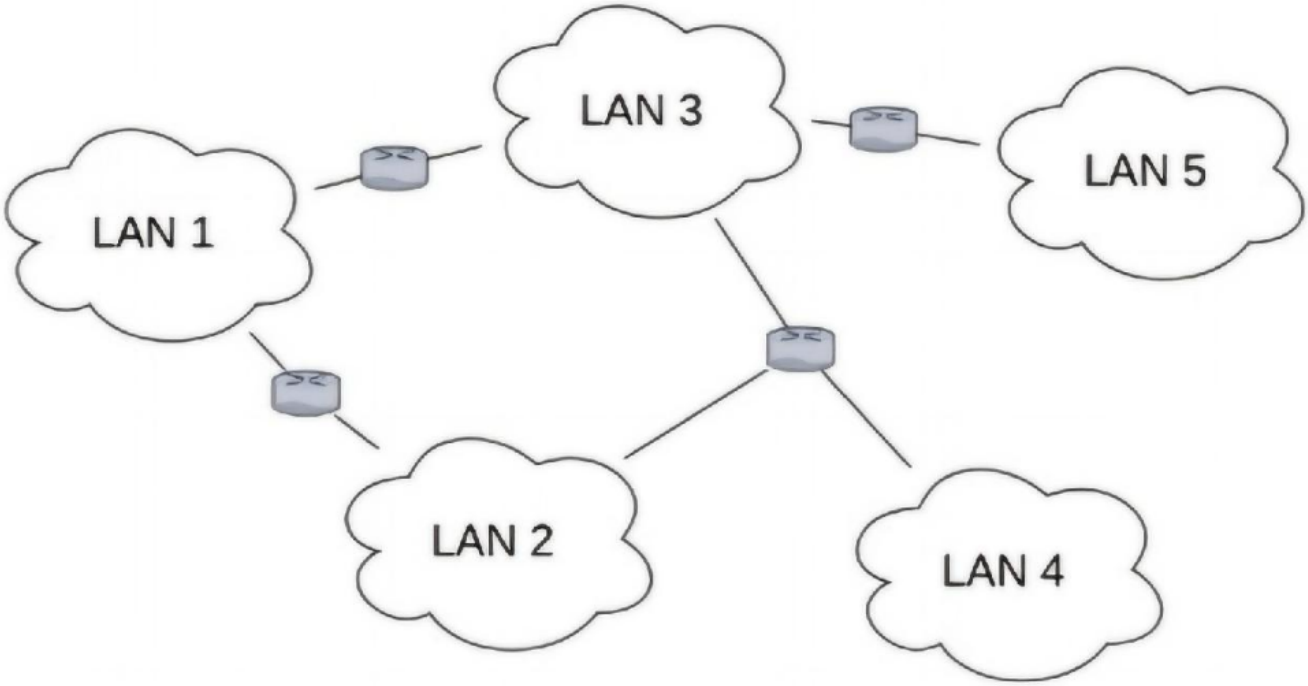
\includegraphics[width=0.75\textwidth]{../figures/esercitazione-es1}
\end{figure}

\noindent
Ci sono due indirizzi già assegnati alla rete:
\begin{itemize}
  \item 101.75.79.255
  \item 101.75.80.0
\end{itemize}

\subsection{Domanda 1}
Qual'è il blocco \textbf{CIDR} più piccolo (con il minor numero di indirizzi) che contiene
tali indirizzi?

\vspace{1em}
\noindent
Converto entrambi gli indirizzi in notazione binaria:
\[
  \begin{aligned}
    101.75.79.255 & \to 01100101 \;\; 01001011 \;\; 01001111 \;\; 11111111 \\
    101.75.80.0   & \to 01100101 \;\; 01001011 \;\; 01010000 \;\; 00000000
  \end{aligned}
\] 
Siccome i due IP sono uguali fino al 19° bit a partire da sinistra, si può dire che
il blocco CIDR più piccolo che contiene entrambi gli indirizzi sia quello della rete:
\[
  \underbrace{01100101 \;\; 01001011 \;\; 010}_{\text{Prefisso}}
  \;\; \underbrace{00000 \;\; 00000000}_{\text{Suffisso}}
\]
che in notazione intera puntata è il seguente:
\[
   101.75.64.0/19
\] 

\subsection{Domanda 2}
Dato il blocco \textbf{CIDR} della domanda precedente, si creino 5 sottoreti con i
seguenti vincoli:
\begin{itemize}
  \item \textbf{LAN 1}: deve essere una sottorete /21

    \vspace{1em}
    \noindent
    Per avere una sottorete /21 basta spostare i bit del prefisso:
    \[
      \underbrace{01100101 \;\; 01001011 \;\; 010}_{\text{Prefisso}}
      \;\; \underbrace{00000 \;\; 00000000}_{\text{Suffisso}}\\
    \]
    \[
      \Downarrow
    \]
    \[
      \underbrace{01100101 \;\; 01001011 \;\; 01000}_{\text{Prefisso}}
      \;\; \underbrace{000 \;\; 00000000}_{\text{Suffisso}}\\
    \] 
    che in notazione intera puntata risulta:
    \[
      101.75.64.0/21
    \] 

  \item \textbf{LAN 2}: deve ospitare fino a 1000 host

    \vspace{1em}
    \noindent
    1000 host sono circa \( 2^{10} \), di conseguenza per avere un blocco che possa
    ospitare fino a 1000 host esso deve avere almeno 10 bit di suffisso:
    \[
      \underbrace{01100101 \;\; 01001011 \;\; 010000}_{\text{Prefisso}}
      \;\; \underbrace{00 \;\; 00000000}_{\text{Suffisso}}\\
    \] 
    che in notazione intera puntata risulta:
    \[
      101.75.64.0/22
    \] 

  \item \textbf{LAN 3}: deve essere una sottorete /23

    \vspace{1em}
    \noindent
    Per avere una sottorete /23 basta spostare i bit del prefisso:
    \[
      \underbrace{01100101 \;\; 01001011 \;\; 010}_{\text{Prefisso}}
      \;\; \underbrace{00000 \;\; 00000000}_{\text{Suffisso}}\\
    \]
    \[
      \Downarrow
    \]
    \[
      \underbrace{01100101 \;\; 01001011 \;\; 0100000}_{\text{Prefisso}}
      \;\; \underbrace{0 \;\; 00000000}_{\text{Suffisso}}\\
    \] 
    che in notazione intera puntata risulta:
    \[
      101.75.64.0/23
    \] 

  \item \textbf{LAN 4}: deve ospitare fino a 400 host

    \vspace{1em}
    \noindent
    400 host sono circa \( 2^{9} \), di conseguenza per avere un blocco che possa
    ospitare fino a 400 host esso deve avere almeno 9 bit di suffisso:
    \[
      \underbrace{01100101 \;\; 01001011 \;\; 0100000}_{\text{Prefisso}}
      \;\; \underbrace{0 \;\; 00000000}_{\text{Suffisso}}\\
    \] 
    che in notazione intera puntata risulta:
    \[
      101.75.64.0/23
    \] 

  \item \textbf{LAN 5}: deve ospitare metà host rispetto al blocco iniziale

    \vspace{1em}
    \noindent
    Il blocco iniziale riesce ad ospitare \( 2^{13} \) host, quindi per creare una rete
    che ne ospiti la metà bisogna avere \( \frac{2^{13}}{2} = 2^{13-1} = 2^{12} \) 12
    bit di suffisso:
    \[
      \underbrace{01100101 \;\; 01001011 \;\; 0100}_{\text{Prefisso}}
      \;\; \underbrace{0000 \;\; 00000000}_{\text{Suffisso}}\\
    \] 
    che in notazione intera puntata risulta:
    \[
      101.75.64.0/20
    \] 
\end{itemize}

\end{document}
